\documentclass[]{book}
\usepackage{lmodern}
\usepackage{amssymb,amsmath}
\usepackage{ifxetex,ifluatex}
\usepackage{fixltx2e} % provides \textsubscript
\ifnum 0\ifxetex 1\fi\ifluatex 1\fi=0 % if pdftex
  \usepackage[T1]{fontenc}
  \usepackage[utf8]{inputenc}
\else % if luatex or xelatex
  \ifxetex
    \usepackage{mathspec}
  \else
    \usepackage{fontspec}
  \fi
  \defaultfontfeatures{Ligatures=TeX,Scale=MatchLowercase}
\fi
% use upquote if available, for straight quotes in verbatim environments
\IfFileExists{upquote.sty}{\usepackage{upquote}}{}
% use microtype if available
\IfFileExists{microtype.sty}{%
\usepackage{microtype}
\UseMicrotypeSet[protrusion]{basicmath} % disable protrusion for tt fonts
}{}
\usepackage{hyperref}
\hypersetup{unicode=true,
            pdftitle={Modelos Predictivos},
            pdfauthor={Freddy Hernández; Olga Usuga; Carmen Patiño},
            pdfborder={0 0 0},
            breaklinks=true}
\urlstyle{same}  % don't use monospace font for urls
\usepackage{natbib}
\bibliographystyle{apalike}
\usepackage{color}
\usepackage{fancyvrb}
\newcommand{\VerbBar}{|}
\newcommand{\VERB}{\Verb[commandchars=\\\{\}]}
\DefineVerbatimEnvironment{Highlighting}{Verbatim}{commandchars=\\\{\}}
% Add ',fontsize=\small' for more characters per line
\usepackage{framed}
\definecolor{shadecolor}{RGB}{248,248,248}
\newenvironment{Shaded}{\begin{snugshade}}{\end{snugshade}}
\newcommand{\AlertTok}[1]{\textcolor[rgb]{0.94,0.16,0.16}{#1}}
\newcommand{\AnnotationTok}[1]{\textcolor[rgb]{0.56,0.35,0.01}{\textbf{\textit{#1}}}}
\newcommand{\AttributeTok}[1]{\textcolor[rgb]{0.77,0.63,0.00}{#1}}
\newcommand{\BaseNTok}[1]{\textcolor[rgb]{0.00,0.00,0.81}{#1}}
\newcommand{\BuiltInTok}[1]{#1}
\newcommand{\CharTok}[1]{\textcolor[rgb]{0.31,0.60,0.02}{#1}}
\newcommand{\CommentTok}[1]{\textcolor[rgb]{0.56,0.35,0.01}{\textit{#1}}}
\newcommand{\CommentVarTok}[1]{\textcolor[rgb]{0.56,0.35,0.01}{\textbf{\textit{#1}}}}
\newcommand{\ConstantTok}[1]{\textcolor[rgb]{0.00,0.00,0.00}{#1}}
\newcommand{\ControlFlowTok}[1]{\textcolor[rgb]{0.13,0.29,0.53}{\textbf{#1}}}
\newcommand{\DataTypeTok}[1]{\textcolor[rgb]{0.13,0.29,0.53}{#1}}
\newcommand{\DecValTok}[1]{\textcolor[rgb]{0.00,0.00,0.81}{#1}}
\newcommand{\DocumentationTok}[1]{\textcolor[rgb]{0.56,0.35,0.01}{\textbf{\textit{#1}}}}
\newcommand{\ErrorTok}[1]{\textcolor[rgb]{0.64,0.00,0.00}{\textbf{#1}}}
\newcommand{\ExtensionTok}[1]{#1}
\newcommand{\FloatTok}[1]{\textcolor[rgb]{0.00,0.00,0.81}{#1}}
\newcommand{\FunctionTok}[1]{\textcolor[rgb]{0.00,0.00,0.00}{#1}}
\newcommand{\ImportTok}[1]{#1}
\newcommand{\InformationTok}[1]{\textcolor[rgb]{0.56,0.35,0.01}{\textbf{\textit{#1}}}}
\newcommand{\KeywordTok}[1]{\textcolor[rgb]{0.13,0.29,0.53}{\textbf{#1}}}
\newcommand{\NormalTok}[1]{#1}
\newcommand{\OperatorTok}[1]{\textcolor[rgb]{0.81,0.36,0.00}{\textbf{#1}}}
\newcommand{\OtherTok}[1]{\textcolor[rgb]{0.56,0.35,0.01}{#1}}
\newcommand{\PreprocessorTok}[1]{\textcolor[rgb]{0.56,0.35,0.01}{\textit{#1}}}
\newcommand{\RegionMarkerTok}[1]{#1}
\newcommand{\SpecialCharTok}[1]{\textcolor[rgb]{0.00,0.00,0.00}{#1}}
\newcommand{\SpecialStringTok}[1]{\textcolor[rgb]{0.31,0.60,0.02}{#1}}
\newcommand{\StringTok}[1]{\textcolor[rgb]{0.31,0.60,0.02}{#1}}
\newcommand{\VariableTok}[1]{\textcolor[rgb]{0.00,0.00,0.00}{#1}}
\newcommand{\VerbatimStringTok}[1]{\textcolor[rgb]{0.31,0.60,0.02}{#1}}
\newcommand{\WarningTok}[1]{\textcolor[rgb]{0.56,0.35,0.01}{\textbf{\textit{#1}}}}
\usepackage{longtable,booktabs}
\usepackage{graphicx,grffile}
\makeatletter
\def\maxwidth{\ifdim\Gin@nat@width>\linewidth\linewidth\else\Gin@nat@width\fi}
\def\maxheight{\ifdim\Gin@nat@height>\textheight\textheight\else\Gin@nat@height\fi}
\makeatother
% Scale images if necessary, so that they will not overflow the page
% margins by default, and it is still possible to overwrite the defaults
% using explicit options in \includegraphics[width, height, ...]{}
\setkeys{Gin}{width=\maxwidth,height=\maxheight,keepaspectratio}
\IfFileExists{parskip.sty}{%
\usepackage{parskip}
}{% else
\setlength{\parindent}{0pt}
\setlength{\parskip}{6pt plus 2pt minus 1pt}
}
\setlength{\emergencystretch}{3em}  % prevent overfull lines
\providecommand{\tightlist}{%
  \setlength{\itemsep}{0pt}\setlength{\parskip}{0pt}}
\setcounter{secnumdepth}{5}
% Redefines (sub)paragraphs to behave more like sections
\ifx\paragraph\undefined\else
\let\oldparagraph\paragraph
\renewcommand{\paragraph}[1]{\oldparagraph{#1}\mbox{}}
\fi
\ifx\subparagraph\undefined\else
\let\oldsubparagraph\subparagraph
\renewcommand{\subparagraph}[1]{\oldsubparagraph{#1}\mbox{}}
\fi

%%% Use protect on footnotes to avoid problems with footnotes in titles
\let\rmarkdownfootnote\footnote%
\def\footnote{\protect\rmarkdownfootnote}

%%% Change title format to be more compact
\usepackage{titling}

% Create subtitle command for use in maketitle
\providecommand{\subtitle}[1]{
  \posttitle{
    \begin{center}\large#1\end{center}
    }
}

\setlength{\droptitle}{-2em}

  \title{Modelos Predictivos}
    \pretitle{\vspace{\droptitle}\centering\huge}
  \posttitle{\par}
    \author{Freddy Hernández \\ Olga Usuga \\ Carmen Patiño}
    \preauthor{\centering\large\emph}
  \postauthor{\par}
      \predate{\centering\large\emph}
  \postdate{\par}
    \date{2019-11-25}

\usepackage{booktabs}
\usepackage[spanish]{babel}
\decimalpoint
\selectlanguage{spanish}

% Comandos para escribir nombres de paquetes, programas y codigos
\newcommand{\pkg}[1]{{\normalfont\fontseries{b}\selectfont #1}}
\let\proglang=\textsf
\let\code=\texttt


\usepackage{booktabs}
\usepackage{longtable}
\usepackage[bf,singlelinecheck=off]{caption}

\usepackage{framed,color}
\definecolor{shadecolor}{RGB}{248,248,248}

\renewcommand{\textfraction}{0.05}
\renewcommand{\topfraction}{0.8}
\renewcommand{\bottomfraction}{0.8}
\renewcommand{\floatpagefraction}{0.75}

\renewenvironment{quote}{\begin{VF}}{\end{VF}}
\let\oldhref\href
\renewcommand{\href}[2]{#2\footnote{\url{#1}}}

\ifxetex
  \usepackage{letltxmacro}
  \setlength{\XeTeXLinkMargin}{1pt}
  \LetLtxMacro\SavedIncludeGraphics\includegraphics
  \def\includegraphics#1#{% #1 catches optional stuff (star/opt. arg.)
    \IncludeGraphicsAux{#1}%
  }%
  \newcommand*{\IncludeGraphicsAux}[2]{%
    \XeTeXLinkBox{%
      \SavedIncludeGraphics#1{#2}%
    }%
  }%
\fi

\makeatletter
\newenvironment{kframe}{%
\medskip{}
\setlength{\fboxsep}{.8em}
 \def\at@end@of@kframe{}%
 \ifinner\ifhmode%
  \def\at@end@of@kframe{\end{minipage}}%
  \begin{minipage}{\columnwidth}%
 \fi\fi%
 \def\FrameCommand##1{\hskip\@totalleftmargin \hskip-\fboxsep
 \colorbox{shadecolor}{##1}\hskip-\fboxsep
     % There is no \\@totalrightmargin, so:
     \hskip-\linewidth \hskip-\@totalleftmargin \hskip\columnwidth}%
 \MakeFramed {\advance\hsize-\width
   \@totalleftmargin\z@ \linewidth\hsize
   \@setminipage}}%
 {\par\unskip\endMakeFramed%
 \at@end@of@kframe}
\makeatother

\renewenvironment{Shaded}{\begin{kframe}}{\end{kframe}}

%%%%%

\newenvironment{rmdblock}[1]
  {
  \begin{itemize}
  \renewcommand{\labelitemi}{
    \raisebox{-.7\height}[0pt][0pt]{
      {\setkeys{Gin}{width=3em,keepaspectratio}\includegraphics{images/#1}}
    }
  }
  \setlength{\fboxsep}{1em}
  \begin{kframe}
  \item
  }
  {
  \end{kframe}
  \end{itemize}
  }
\newenvironment{rmdnote}
  {\begin{rmdblock}{note}}
  {\end{rmdblock}}
\newenvironment{rmdcaution}
  {\begin{rmdblock}{caution}}
  {\end{rmdblock}}
\newenvironment{rmdimportant}
  {\begin{rmdblock}{important}}
  {\end{rmdblock}}
\newenvironment{rmdtip}
  {\begin{rmdblock}{tip}}
  {\end{rmdblock}}
\newenvironment{rmdwarning}
  {\begin{rmdblock}{warning}}
  {\end{rmdblock}}


%%%%%


\usepackage{makeidx}
\makeindex

\urlstyle{tt}

\usepackage{amsthm}
\makeatletter
\def\thm@space@setup{%
  \thm@preskip=8pt plus 2pt minus 4pt
  \thm@postskip=\thm@preskip
}
\makeatother

\frontmatter

\let\BeginKnitrBlock\begin \let\EndKnitrBlock\end
\begin{document}
\maketitle

% you may need to leave a few empty pages before the dedication page

%\cleardoublepage\newpage\thispagestyle{empty}\null
%\cleardoublepage\newpage\thispagestyle{empty}\null
%\cleardoublepage\newpage
\thispagestyle{empty}

\begin{center}

Gracias a Dios por todo lo que me ha dado.

%\includegraphics{images/dedication.pdf}
\end{center}

\setlength{\abovedisplayskip}{-5pt}
\setlength{\abovedisplayshortskip}{-5pt}

{
\setcounter{tocdepth}{1}
\tableofcontents
}
\hypertarget{bienvenido}{%
\chapter*{Bienvenido}\label{bienvenido}}
\addcontentsline{toc}{chapter}{Bienvenido}

\begin{center}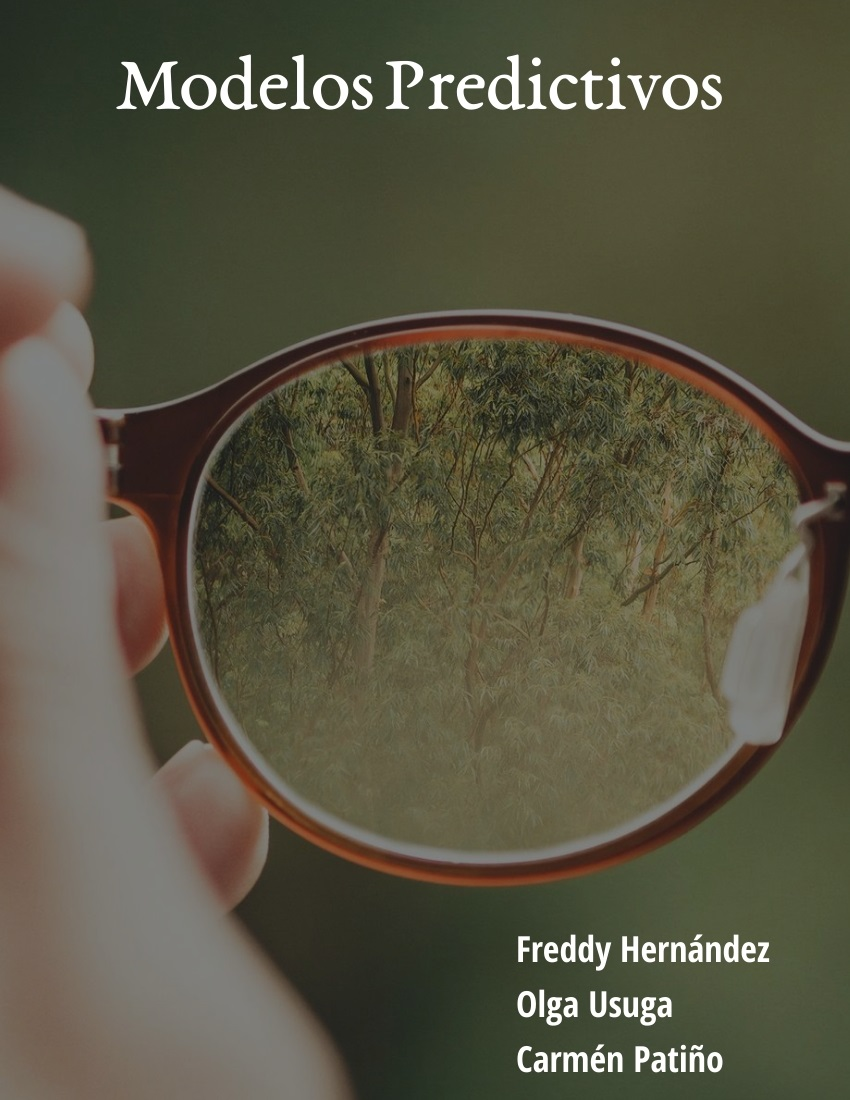
\includegraphics[width=0.5\linewidth]{images/cover} \end{center}

Este libro está destinado para estudiantes de ingeniería y estadística que deseen aprender sobre modelos de regresión y la forma de aplicarlos por medio del lenguaje de programación R.

\href{https://fhernanb.github.io/}{Freddy Hernández}\\
\href{http://scienti.colciencias.gov.co:8081/cvlac/visualizador/generarCurriculoCv.do?cod_rh=0001417591}{Olga Usuga}\\
\href{http://scienti.colciencias.gov.co:8081/cvlac/visualizador/generarCurriculoCv.do?cod_rh=0000756008}{Carmen Patiño}

\hypertarget{estructura-del-libro}{%
\section*{Estructura del libro}\label{estructura-del-libro}}
\addcontentsline{toc}{section}{Estructura del libro}

En el capítulo \ref{arb-de-regre} se presentan los árboles de regresión.

\hypertarget{software-y-convenciones}{%
\section*{Software y convenciones}\label{software-y-convenciones}}
\addcontentsline{toc}{section}{Software y convenciones}

Para realizar este libro usamos los paquetes \textbf{knitr}\index{knitr} \citep{xie2015} y \textbf{bookdown}\index{bookdown} \citep{R-bookdown} que permiten unir la ventajas de LaTeX y R en un mismo archivo.

En todo el libro se presentarán códigos que el lector puede copiar y pegar en su consola de R para obtener los mismos resultados aquí del libro. Los códigos se destacan en una caja de color similar a la mostrada a continuación.

\begin{Shaded}
\begin{Highlighting}[]
\DecValTok{4} \OperatorTok{+}\StringTok{ }\DecValTok{6}
\NormalTok{a <-}\StringTok{ }\KeywordTok{c}\NormalTok{(}\DecValTok{1}\NormalTok{, }\DecValTok{5}\NormalTok{, }\DecValTok{6}\NormalTok{)}
\DecValTok{5} \OperatorTok{*}\StringTok{ }\NormalTok{a}
\DecValTok{1}\OperatorTok{:}\DecValTok{10}
\end{Highlighting}
\end{Shaded}

Los resultados o salidas obtenidos de cualquier código se destacan con dos símbolos de númeral (\texttt{\#\#}) al inicio de cada línea o renglón, esto quiere decir que todo lo que inicie con \texttt{\#\#} son resultados obtenidos y \textbf{NO} los debe copiar. Abajo se muestran los resultados obtenidos luego de correr el código anterior.

\begin{verbatim}
## [1] 10
\end{verbatim}

\begin{verbatim}
## [1]  5 25 30
\end{verbatim}

\begin{verbatim}
##  [1]  1  2  3  4  5  6  7  8  9 10
\end{verbatim}

\hypertarget{bloques-informativos}{%
\section*{Bloques informativos}\label{bloques-informativos}}
\addcontentsline{toc}{section}{Bloques informativos}

En varias partes del libro usaremos bloques informativos para resaltar algún aspecto importante. Abajo se encuentra un ejemplo de los bloques y su significado.

\BeginKnitrBlock{rmdnote}
Nota aclaratoria.
\EndKnitrBlock{rmdnote}

\BeginKnitrBlock{rmdtip}
Sugerencia.
\EndKnitrBlock{rmdtip}

\BeginKnitrBlock{rmdwarning}
Advertencia.
\EndKnitrBlock{rmdwarning}

\hypertarget{arb-de-regre}{%
\chapter{Árboles de regresión}\label{arb-de-regre}}

Los árboles de regresión/clasificación fueron propuestos par \href{https://en.wikipedia.org/wiki/Leo_Breiman}{Leo Breiman} en el libro \citep{Breiman1984} y son árboles de decisión que tienen como objetivo asignar un valor de \(\hat{y}\) dependiendo de los valores de las covariables.

Los árboles se pueden clasificar en dos tipos que son:

\begin{enumerate}
\def\labelenumi{\arabic{enumi}.}
\tightlist
\item
  Árboles de regresión en los cuales la variable respuesta \(y\) es cuantitativa.
\item
  Árboles de clasificación en los cuales la variable respuesta \(y\) es cualitativa.
\end{enumerate}

El presente capítulo está destinado a árboles de regresión, los árboles de clasificación se explican en el capítulo \ref{arb-de-clasif}.

Un árbol de regresión consiste en hacer preguntas de tipo ¿\(x_k \leq c\)? para cada una de las covariables, de esta forma el espacio de las covariables es divido en hiper-rectángulos y todas las observaciones que queden dentro de un hiper-rectángulo tendrán el mismo valor estimado \(\hat{y}\).

En la siguiente figura se ilustra el árbol en el lado izquierdo y la partición del espacio en el lado derecho. La partición del espacio se hace de manera repetitiva para encontrar las variables y los valores de corte \(c\) de tal manera que se minimice la función de costos \(\sum_{i=1}^{i=n} (y_i - \hat{y}_i)^2\).

\begin{figure}

{\centering 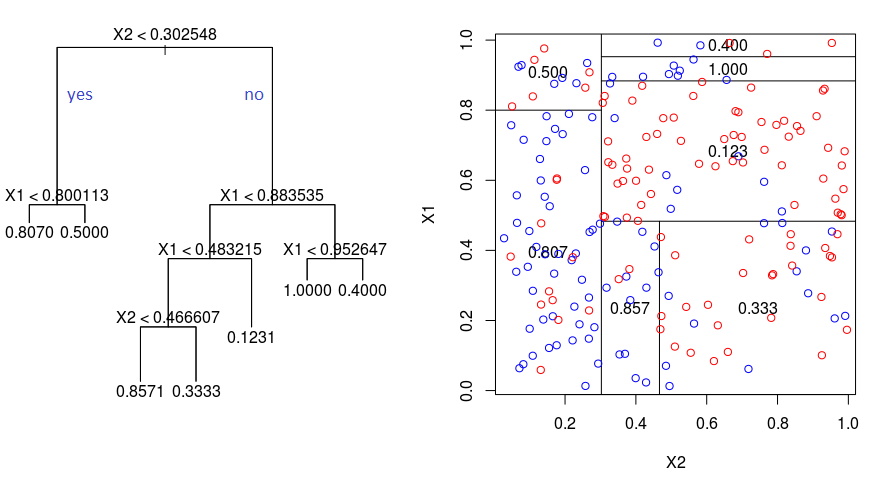
\includegraphics[width=21.77in]{images/ilustracion_arb_regresion} 

}

\caption{Ilustración de la técnica Árboles de Regresión. A la izquierda el árbol y a la derecha la partición del espacio.}\label{fig:ilustra-arbol-reg01}
\end{figure}

Los pasos para realizar la partición del espacio son:

\begin{enumerate}
\def\labelenumi{\arabic{enumi}.}
\tightlist
\item
  Dado un conjunto de covariables (características), encontrar la covariable que permita predecir mejor la variable respuesta.
\item
  Encontrar el punto de corte \(c\) sobre esa covariable que permita predecir mejor la variable respuesta.
\item
  Repetir los pasos anteriores hasta que se alcance el criterio de parada.
\end{enumerate}

Algunas de las ventajas de los árboles de regresión son:

\begin{itemize}
\tightlist
\item
  Fácil de entender e intrepretar.
\item
  Requiere poca preparación de los datos.
\item
  Las covariables pueden ser cualitativas o cuantitativas.
\item
  No exige supuestos distribucionales.
\end{itemize}

Para explicaciones más detalladas sobre las técnicas basadas en árboles recomendamos consultar el capítulo 8 de \citep{james2013}. Se recomienda también ver \href{https://www.youtube.com/watch?v=7VeUPuFGJHk}{este video} con una explicación sencilla sobre árboles.

\hypertarget{paquetes}{%
\section*{Paquetes}\label{paquetes}}
\addcontentsline{toc}{section}{Paquetes}

En esta sección se mencionan algunos de los paquetes más comunes para implementar árboles de regresión.

El paquete \textbf{rpart} \citep{R-rpart} es uno de los paquetes que se pueden usar para crear árboles de regresión. La función para crear un árbol de regresión es \texttt{rpart}, a continuación la estructura de la función.

\begin{Shaded}
\begin{Highlighting}[]
\KeywordTok{rpart}\NormalTok{(formula, data, weights, subset, }\DataTypeTok{na.action =}\NormalTok{ na.rpart, method,}
      \DataTypeTok{model =} \OtherTok{FALSE}\NormalTok{, }\DataTypeTok{x =} \OtherTok{FALSE}\NormalTok{, }\DataTypeTok{y =} \OtherTok{TRUE}\NormalTok{, parms, control, cost, ...)}
\end{Highlighting}
\end{Shaded}

Otro paquete útil para árboles de regresión es \textbf{tree} \citep{R-tree}. La función para crear un árbol de regresión es \texttt{tree}, a continuación la estructura de la función.

\begin{Shaded}
\begin{Highlighting}[]
\KeywordTok{tree}\NormalTok{(formula, data, weights, subset,}
     \DataTypeTok{na.action =}\NormalTok{ na.pass, }\DataTypeTok{control =} \KeywordTok{tree.control}\NormalTok{(nobs, ...),}
     \DataTypeTok{method =} \StringTok{"recursive.partition"}\NormalTok{,}
     \DataTypeTok{split =} \KeywordTok{c}\NormalTok{(}\StringTok{"deviance"}\NormalTok{, }\StringTok{"gini"}\NormalTok{),}
     \DataTypeTok{model =} \OtherTok{FALSE}\NormalTok{, }\DataTypeTok{x =} \OtherTok{FALSE}\NormalTok{, }\DataTypeTok{y =} \OtherTok{TRUE}\NormalTok{, }\DataTypeTok{wts =} \OtherTok{TRUE}\NormalTok{, ...)}
\end{Highlighting}
\end{Shaded}

\BeginKnitrBlock{rmdnote}
Se recomienda al lector que consulte la ayuda de las funciones anteriores para que pueda entender las posibilidades que se tienen con cada una de ellas.
\EndKnitrBlock{rmdnote}

\hypertarget{ejemplo-con-el-paquete-rpart}{%
\section*{\texorpdfstring{Ejemplo con el paquete \textbf{rpart}}{Ejemplo con el paquete rpart}}\label{ejemplo-con-el-paquete-rpart}}
\addcontentsline{toc}{section}{Ejemplo con el paquete \textbf{rpart}}

En este ejemplo se busca encontrar un modelo de regresion lineal que explique la variable respuesta \(y\) en función de las covariables \(x_1\) a \(x_{11}\), los datos provienen del ejercicio 9.5 del libro de \href{https://www.amazon.com/Introduccion-analisis-regresion-lineal-Spanish/dp/9702403278}{Montgomery, Peck and Vining (2003)}. El paquete \textbf{MPV} \citep{R-MPV} contiene todos los datos que acompañan al libro.

A continuación se muestra el encabezado de la base de datos y la definición de las variables.

\begin{figure}

{\centering 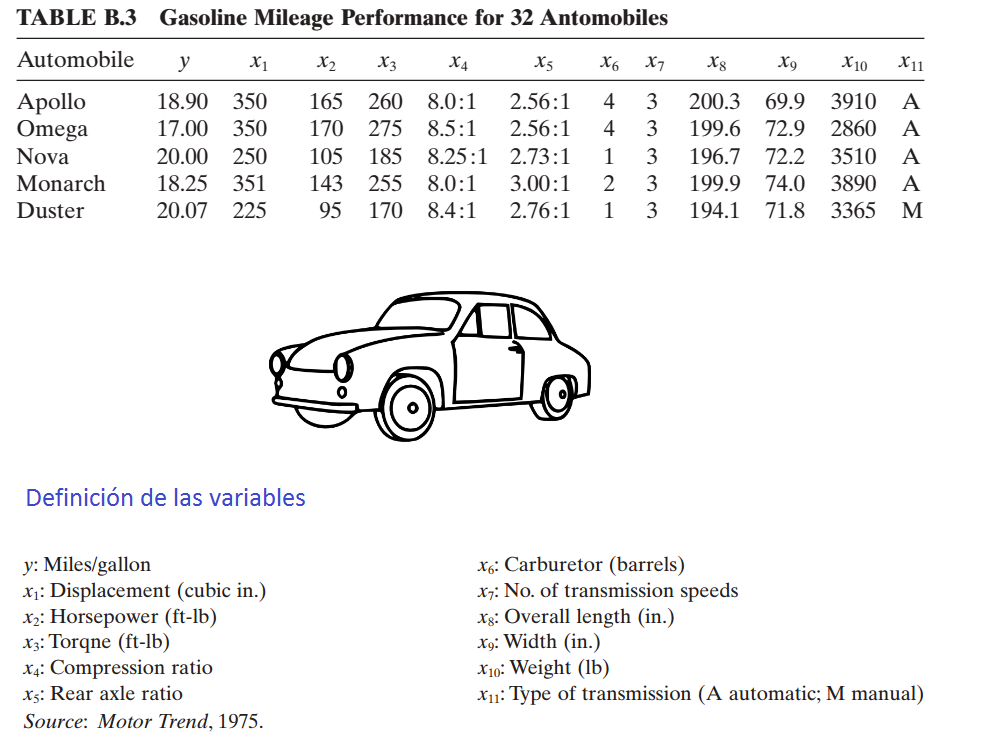
\includegraphics[width=24.55in]{images/tableb3} 

}

\caption{Ilustración de la base de datos.}\label{fig:selection02}
\end{figure}

\textbf{Nota}: Type of transmission (1=automatic, 0=manual).

Antes de iniciar es necesario revisar si hay \texttt{NA\textquotesingle{}s} y eliminarlos.

\begin{Shaded}
\begin{Highlighting}[]
\KeywordTok{library}\NormalTok{(MPV)  }\CommentTok{# Aqui estan los datos}
\NormalTok{table.b3[}\DecValTok{22}\OperatorTok{:}\DecValTok{26}\NormalTok{, ] }\CommentTok{# Can you see the missing values?}
\end{Highlighting}
\end{Shaded}

\begin{verbatim}
##        y    x1  x2  x3  x4   x5 x6 x7    x8   x9  x10 x11
## 22 21.47 360.0 180 290 8.4 2.45  2  3 214.2 76.3 4250   1
## 23 16.59 400.0 185  NA 7.6 3.08  4  3 196.0 73.0 3850   1
## 24 31.90  96.9  75  83 9.0 4.30  2  5 165.2 61.8 2275   0
## 25 29.40 140.0  86  NA 8.0 2.92  2  4 176.4 65.4 2150   0
## 26 13.27 460.0 223 366 8.0 3.00  4  3 228.0 79.8 5430   1
\end{verbatim}

\begin{Shaded}
\begin{Highlighting}[]
\NormalTok{datos <-}\StringTok{ }\NormalTok{table.b3[}\OperatorTok{-}\KeywordTok{c}\NormalTok{(}\DecValTok{23}\NormalTok{, }\DecValTok{25}\NormalTok{), ]}
\end{Highlighting}
\end{Shaded}

El objeto \texttt{datos} tiene la base de datos sin las líneas con \texttt{NA}, lo mismo se hubiese podido realizar usando la función \texttt{na.omit}. La base de datos tiene 30 filas y 12 columnas.

\begin{Shaded}
\begin{Highlighting}[]
\KeywordTok{library}\NormalTok{(rpart)}
\KeywordTok{library}\NormalTok{(rpart.plot)}
\end{Highlighting}
\end{Shaded}

\begin{Shaded}
\begin{Highlighting}[]
\NormalTok{mod1 <-}\StringTok{ }\KeywordTok{rpart}\NormalTok{(y }\OperatorTok{~}\StringTok{ }\NormalTok{., }\DataTypeTok{data=}\NormalTok{datos)}
\end{Highlighting}
\end{Shaded}

Dibjuemos el árbol con \texttt{prp} que es una función del paquete \textbf{rpart.plot} \citep{R-rpart.plot}.

\begin{Shaded}
\begin{Highlighting}[]
\KeywordTok{prp}\NormalTok{(mod1)}
\end{Highlighting}
\end{Shaded}

\begin{center}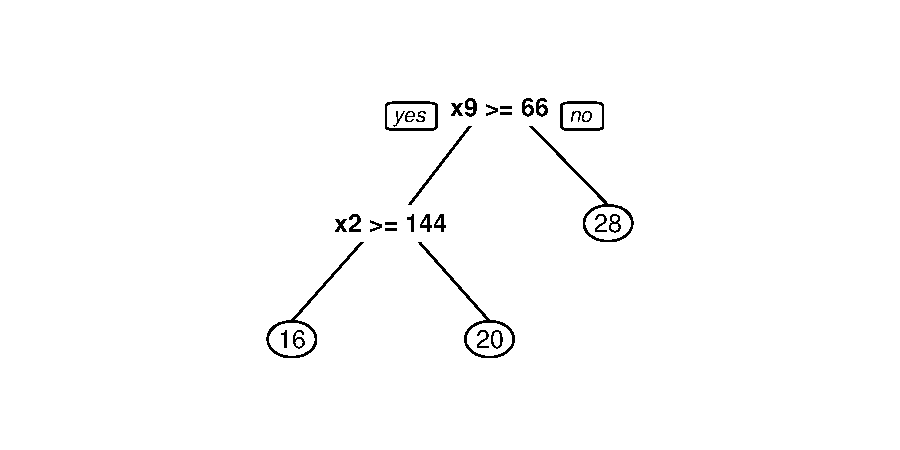
\includegraphics{libro_mod_pred_files/figure-latex/arbol01-1} \end{center}

Construyamos nuevamente el árbol pero explorando todas las opciones de la función \texttt{prp}.

\begin{Shaded}
\begin{Highlighting}[]
\KeywordTok{prp}\NormalTok{(mod1, }\DataTypeTok{main=}\StringTok{""}\NormalTok{,}
    \DataTypeTok{nn =} \OtherTok{TRUE}\NormalTok{,             }\CommentTok{# display the node numbers}
    \DataTypeTok{fallen.leaves =} \OtherTok{TRUE}\NormalTok{,  }\CommentTok{# put the leaves on the bottom of the page}
    \DataTypeTok{shadow.col =} \StringTok{"gray"}\NormalTok{,   }\CommentTok{# shadows under the leaves}
    \DataTypeTok{branch.lty =} \DecValTok{3}\NormalTok{,        }\CommentTok{# draw branches using dotted lines}
    \DataTypeTok{branch =} \FloatTok{.5}\NormalTok{,           }\CommentTok{# change angle of branch lines}
    \DataTypeTok{faclen =} \DecValTok{0}\NormalTok{,            }\CommentTok{# faclen = 0 to print full factor names}
    \DataTypeTok{trace =} \DecValTok{1}\NormalTok{,             }\CommentTok{# print the auto calculated cex, xlim, ylim}
    \DataTypeTok{split.cex =} \FloatTok{1.2}\NormalTok{,       }\CommentTok{# make the split text larger than the node text}
    \DataTypeTok{split.prefix =} \StringTok{"is "}\NormalTok{,  }\CommentTok{# put "is " before split text}
    \DataTypeTok{split.suffix =} \StringTok{"?"}\NormalTok{,    }\CommentTok{# put "?" after split text}
    \DataTypeTok{split.box.col =} \StringTok{"lightblue"}\NormalTok{,   }\CommentTok{# lightgray split boxes (default is white)}
    \DataTypeTok{split.border.col =} \StringTok{"darkgray"}\NormalTok{, }\CommentTok{# darkgray border on split boxes}
    \DataTypeTok{split.round =} \FloatTok{0.5}\NormalTok{)             }\CommentTok{# round the split box corners a tad}
\end{Highlighting}
\end{Shaded}

\begin{verbatim}
## cex 1   xlim c(0, 1)   ylim c(0, 1)
\end{verbatim}

\begin{center}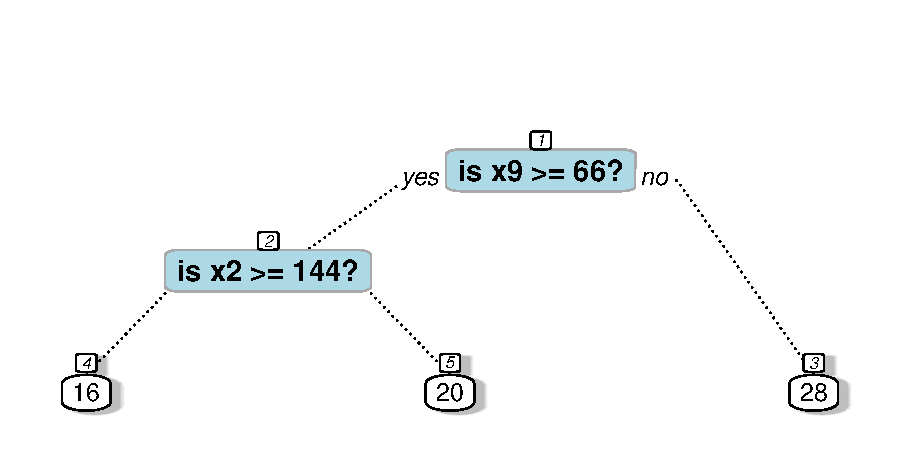
\includegraphics{libro_mod_pred_files/figure-latex/arbol02-1} \end{center}

Usando la información del árbol anterior es posible predecir el valor de \(y\). Por ejemplo:

\begin{enumerate}
\def\labelenumi{\arabic{enumi}.}
\tightlist
\item
  Si una nueva observación tiene \(x_9=70\) y \(x_2=100\), entonces \(\hat{y}=20\).
\item
  Si otra observación tiene \(x_9=60\) y \(x_2=150\), entonces \(\hat{y}=28\).
\end{enumerate}

Como en el árbol anterior solo aparecen las variables \(x_2\) y \(x_9\) se recomienda volver a construir el árbol sólo con ellas.

\begin{Shaded}
\begin{Highlighting}[]
\NormalTok{mod1 <-}\StringTok{ }\KeywordTok{rpart}\NormalTok{(y }\OperatorTok{~}\StringTok{ }\NormalTok{x2 }\OperatorTok{+}\StringTok{ }\NormalTok{x9, }\DataTypeTok{data=}\NormalTok{datos)}
\end{Highlighting}
\end{Shaded}

Este árbol por tener solo dos covariables se puede representar de la siguiente forma:

\begin{Shaded}
\begin{Highlighting}[]
\KeywordTok{with}\NormalTok{(datos, }\KeywordTok{plot}\NormalTok{(}\DataTypeTok{x=}\NormalTok{x2, }\DataTypeTok{y=}\NormalTok{x9))}
\KeywordTok{abline}\NormalTok{(}\DataTypeTok{h=}\DecValTok{66}\NormalTok{, }\DataTypeTok{lty=}\StringTok{'dashed'}\NormalTok{, }\DataTypeTok{col=}\StringTok{'blue'}\NormalTok{)}
\KeywordTok{segments}\NormalTok{(}\DataTypeTok{x0=}\DecValTok{144}\NormalTok{, }\DataTypeTok{y0=}\DecValTok{66}\NormalTok{, }\DataTypeTok{x1=}\DecValTok{144}\NormalTok{, }\DataTypeTok{y1=}\DecValTok{82}\NormalTok{, }\DataTypeTok{lty=}\StringTok{'dashed'}\NormalTok{, }\DataTypeTok{col=}\StringTok{'blue'}\NormalTok{)}
\KeywordTok{text}\NormalTok{(}\DataTypeTok{x=}\DecValTok{120}\NormalTok{, }\DataTypeTok{y=}\DecValTok{63}\NormalTok{, }\DataTypeTok{labels=}\StringTok{'y=28'}\NormalTok{, }\DataTypeTok{col=}\DecValTok{4}\NormalTok{)}
\KeywordTok{text}\NormalTok{(}\DataTypeTok{x=}\DecValTok{90}\NormalTok{, }\DataTypeTok{y=}\DecValTok{73}\NormalTok{, }\DataTypeTok{labels=}\StringTok{'y=20'}\NormalTok{, }\DataTypeTok{col=}\DecValTok{4}\NormalTok{)}
\KeywordTok{text}\NormalTok{(}\DataTypeTok{x=}\DecValTok{190}\NormalTok{, }\DataTypeTok{y=}\DecValTok{73}\NormalTok{, }\DataTypeTok{labels=}\StringTok{'y=16'}\NormalTok{, }\DataTypeTok{col=}\DecValTok{4}\NormalTok{)}
\end{Highlighting}
\end{Shaded}

\begin{center}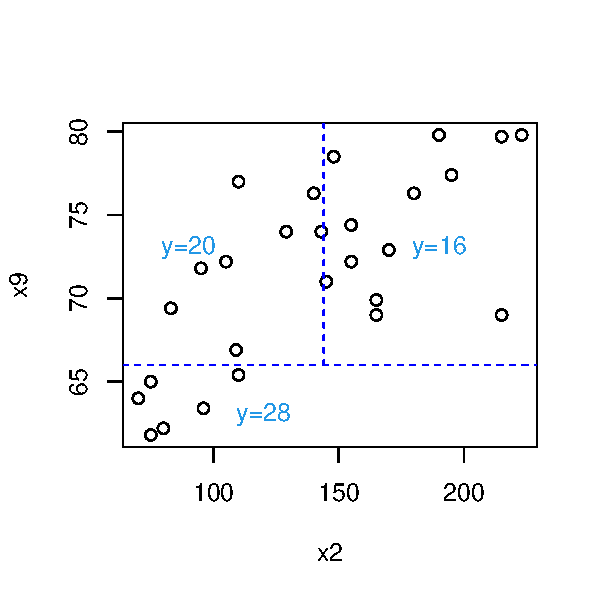
\includegraphics{libro_mod_pred_files/figure-latex/arbol03-1} \end{center}

Para predecir los valores de \(y\) se puede usar la función \texttt{predict}. A continuación el código para predecir la respuesta en los dos casos anteriores.

\begin{Shaded}
\begin{Highlighting}[]
\NormalTok{nuevos_datos <-}\StringTok{ }\KeywordTok{data.frame}\NormalTok{(}\DataTypeTok{x2=}\KeywordTok{c}\NormalTok{(}\DecValTok{100}\NormalTok{, }\DecValTok{150}\NormalTok{), }\DataTypeTok{x9=}\KeywordTok{c}\NormalTok{(}\DecValTok{70}\NormalTok{, }\DecValTok{60}\NormalTok{))}
\KeywordTok{predict}\NormalTok{(}\DataTypeTok{object=}\NormalTok{mod1, }\DataTypeTok{newdata=}\NormalTok{nuevos_datos)}
\end{Highlighting}
\end{Shaded}

\begin{verbatim}
##        1        2 
## 19.66875 28.06625
\end{verbatim}

En este ejemplo los datos originales se usaron como conjunto de entrenamiento y prueba debido a que solo se cuentan con 30 observaciones.

Entre más cerca estén las \(\hat{y}\) de los \(y\) observados se puede decir que el modelo es mejor. A continuación la correlación entre \(\hat{y}\) y \(y\).

\begin{Shaded}
\begin{Highlighting}[]
\NormalTok{y_hat <-}\StringTok{ }\KeywordTok{predict}\NormalTok{(}\DataTypeTok{object=}\NormalTok{mod1, }\DataTypeTok{newdata=}\NormalTok{datos)}
\KeywordTok{cor}\NormalTok{(y_hat, datos}\OperatorTok{$}\NormalTok{y)}
\end{Highlighting}
\end{Shaded}

\begin{verbatim}
## [1] 0.8300304
\end{verbatim}

¿Qué opina de este valor?

A continuación un diagrama de dispersión entre \(\hat{y}\) y \(y\).

\begin{Shaded}
\begin{Highlighting}[]
\KeywordTok{plot}\NormalTok{(}\DataTypeTok{x=}\NormalTok{datos}\OperatorTok{$}\NormalTok{y, }\DataTypeTok{y=}\NormalTok{y_hat, }\DataTypeTok{pch=}\DecValTok{20}\NormalTok{, }\DataTypeTok{las=}\DecValTok{1}\NormalTok{, }\DataTypeTok{xlab=}\StringTok{'y'}\NormalTok{, }\DataTypeTok{ylab=}\KeywordTok{expression}\NormalTok{(}\KeywordTok{hat}\NormalTok{(y)))}
\KeywordTok{abline}\NormalTok{(}\DataTypeTok{a=}\DecValTok{0}\NormalTok{, }\DataTypeTok{b=}\DecValTok{1}\NormalTok{, }\DataTypeTok{lty=}\StringTok{"dashed"}\NormalTok{, }\DataTypeTok{col=}\StringTok{"blue"}\NormalTok{)}
\end{Highlighting}
\end{Shaded}

\begin{center}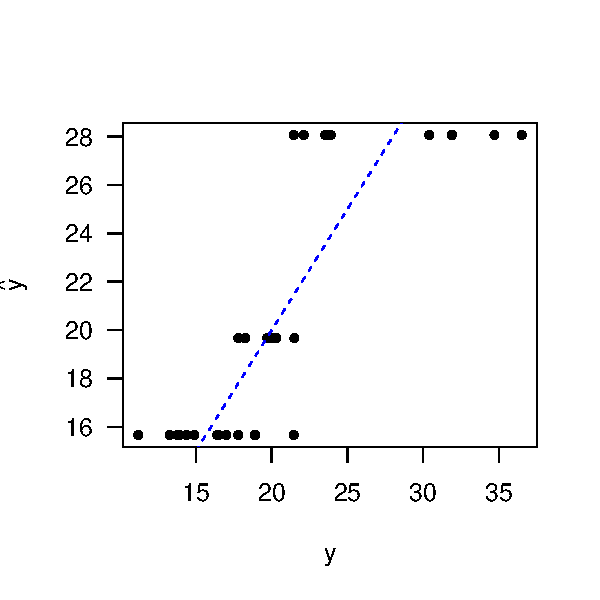
\includegraphics{libro_mod_pred_files/figure-latex/arbol04-1} \end{center}

\hypertarget{ejemplo-con-el-paquete-tree}{%
\section*{\texorpdfstring{Ejemplo con el paquete \textbf{tree}}{Ejemplo con el paquete tree}}\label{ejemplo-con-el-paquete-tree}}
\addcontentsline{toc}{section}{Ejemplo con el paquete \textbf{tree}}

Aquí vamos a repetir el ejemplo anterior con otro paquete.

\begin{Shaded}
\begin{Highlighting}[]
\KeywordTok{library}\NormalTok{(tree)}
\NormalTok{mod2 <-}\StringTok{ }\KeywordTok{tree}\NormalTok{(y }\OperatorTok{~}\StringTok{ }\NormalTok{., }\DataTypeTok{data=}\NormalTok{datos)}
\end{Highlighting}
\end{Shaded}

Para dibujar el árbol se puede usar las siguientes instrucciones.

\begin{Shaded}
\begin{Highlighting}[]
\KeywordTok{plot}\NormalTok{(mod2)}
\KeywordTok{text}\NormalTok{(mod2, }\DataTypeTok{pretty=}\DecValTok{0}\NormalTok{)}
\end{Highlighting}
\end{Shaded}

\begin{center}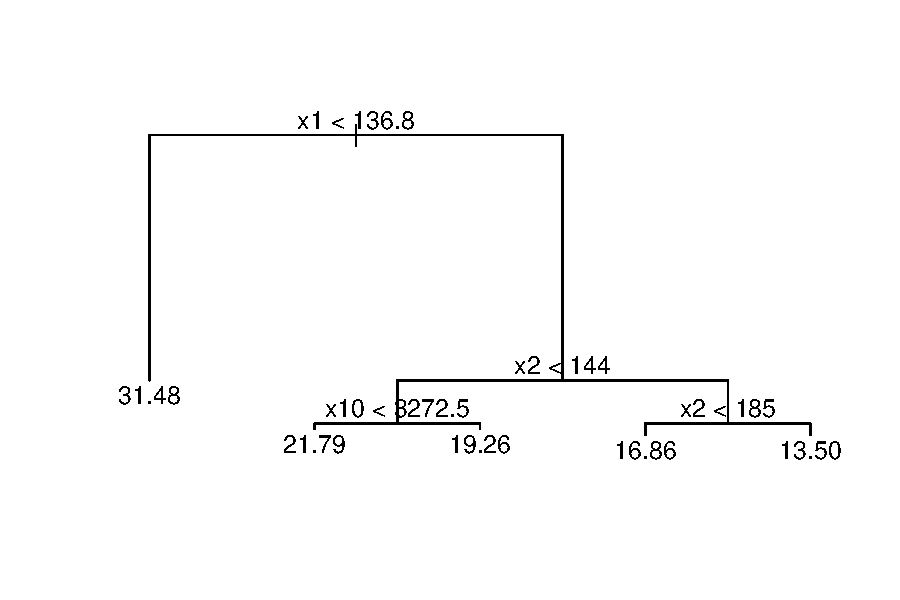
\includegraphics{libro_mod_pred_files/figure-latex/tree01-1} \end{center}

Entre más cerca estén las \(\hat{y}\) de los \(y\) observados se puede decir que el modelo es mejor. A continuación la correlación entre \(\hat{y}\) y \(y\).

\begin{Shaded}
\begin{Highlighting}[]
\NormalTok{y_hat <-}\StringTok{ }\KeywordTok{predict}\NormalTok{(}\DataTypeTok{object=}\NormalTok{mod2, }\DataTypeTok{newdata=}\NormalTok{datos)}
\KeywordTok{cor}\NormalTok{(y_hat, datos}\OperatorTok{$}\NormalTok{y)}
\end{Highlighting}
\end{Shaded}

\begin{verbatim}
## [1] 0.9265051
\end{verbatim}

\hypertarget{arb-de-clasif}{%
\chapter{Árboles de clasificación}\label{arb-de-clasif}}

Los árboles de regresión/clasificación fueron propuestos par \href{https://en.wikipedia.org/wiki/Leo_Breiman}{Leo Breiman} en el libro \citep{Breiman1984} y son árboles de decisión que tienen como objetivo asignar un valor de \(\hat{y}\) dependiendo de los valores de las covariables.

Los árboles se pueden clasificar en dos tipos que son:

\begin{enumerate}
\def\labelenumi{\arabic{enumi}.}
\tightlist
\item
  Árboles de regresión en los cuales la variable respuesta \(y\) es cuantitativa.
\item
  Árboles de clasificación en los cuales la variable respuesta \(y\) es cualitativa.
\end{enumerate}

El presente capítulo está destinado a árboles de clasificación, los árboles de regresión se explican en el capítulo \ref{arb-de-regre}.

\hypertarget{svm-clas}{%
\chapter{Support Vector Machines}\label{svm-clas}}

\citet{Cortes1995} propusieron las máquinas de soporte vectorial para el problema de clasificación.

Suponga que deseamos tenemos dos grupos de objetos, unos de color rojo y otros de color amarillo como se muestran en la siguiente figura.

\begin{figure}

{\centering 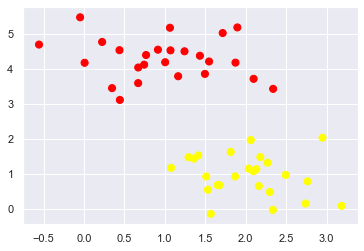
\includegraphics[width=9.1in]{images/svm_1} 

}

\caption{Ilustración de la técnica Árboles de Regresión. A la izquierda el árbol y a la derecha la partición del espacio.}\label{fig:svmreg1}
\end{figure}

El objetivo es dibujar una línea recta que separe los dos grupos, sin embargo, muchas líneas se podrían dibujar, a continuación se muestran tres posibles líneas con las cuales se consigue el objetivo.

\begin{figure}

{\centering 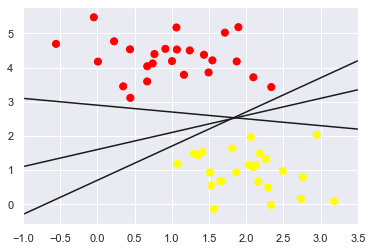
\includegraphics[width=9.3in]{images/svm_2} 

}

\caption{espacio2.}\label{fig:svmreg2}
\end{figure}

Imaginemos que cada línea es como una carretera que se puede ampliar a ambos lados hasta que toque el punto más cercano, ya se amarillo o rojo. Al hacer esto vamos a obtener las tres carreteras que se muestran a continuación.

\begin{figure}

{\centering 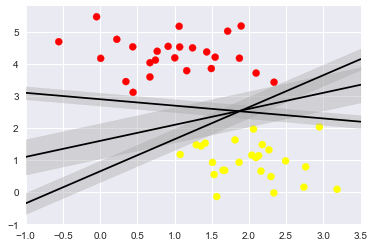
\includegraphics[width=9.35in]{images/svm_3} 

}

\caption{espacio3.}\label{fig:svmreg3}
\end{figure}

De todas las carreteras nos interesa aquella que tenga el mayor ancho o margen, con esa carretera es que se pueden clasificar nuevas observaciones en el grupo rojo o grupo amarillo. A continuación se muestra la figura sólo con la línea de separación que tiene el mayor ancho.

\begin{figure}

{\centering 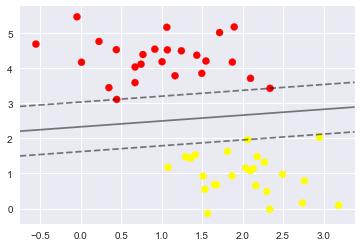
\includegraphics[width=9.03in]{images/svm_4} 

}

\caption{espacio4.}\label{fig:svmreg4}
\end{figure}

\hypertarget{reg-versus-arb}{%
\chapter{Regresión lineal versus árboles de regresión}\label{reg-versus-arb}}

En este capítulo se muestra una comparación entre modelos de regresión y árboles de regresion.

\hypertarget{regresion-lineal}{%
\section*{Regresión lineal}\label{regresion-lineal}}
\addcontentsline{toc}{section}{Regresión lineal}

El modelo de regresión lineal simple es uno de los más populares en modelación. Este modelo se puede resumir a continuación.

\begin{align}
y_i &\sim N(\mu_i, \sigma^2), \\ 
\mu_i &= \beta_0 + \beta_1 x_i, \\
\sigma^2 &= \text{constante}
\end{align}

\hypertarget{arboles-de-regresion}{%
\section*{Arboles de regresión}\label{arboles-de-regresion}}
\addcontentsline{toc}{section}{Arboles de regresión}

Una explicación de los árboles de regresión puede ser consultada en el capítulo \ref{arb-de-regre}.

Las librerías en R para implementar árboles de regresión son:

\begin{Shaded}
\begin{Highlighting}[]
\KeywordTok{library}\NormalTok{(rpart)}
\KeywordTok{library}\NormalTok{(rpart.plot)}
\end{Highlighting}
\end{Shaded}

\hypertarget{ejemplo}{%
\section*{Ejemplo}\label{ejemplo}}
\addcontentsline{toc}{section}{Ejemplo}

Como ilustración vamos a usar los datos del ejemplo 2.1 del libro de \href{https://www.amazon.com/Introduccion-analisis-regresion-lineal-Spanish/dp/9702403278}{Montgomery, Peck and Vining (2003)}. En el ejemplo 2.1 los autores ajustaron un modelo de regresión lineal simple para explicar la Resistencia de una soldadura en función de la Edad de la misma.

A continuación el código para cargar los datos y una muestra de las 6 primeras observaciones de la base de datos, en total tenemos 20 observaciones.

\begin{Shaded}
\begin{Highlighting}[]
\NormalTok{file <-}\StringTok{ "https://raw.githubusercontent.com/fhernanb/datos/master/propelente"}
\NormalTok{datos <-}\StringTok{ }\KeywordTok{read.table}\NormalTok{(}\DataTypeTok{file=}\NormalTok{file, }\DataTypeTok{header=}\OtherTok{TRUE}\NormalTok{)}
\KeywordTok{head}\NormalTok{(datos) }\CommentTok{# shows the first 6 rows}
\end{Highlighting}
\end{Shaded}

\begin{verbatim}
##   Resistencia  Edad
## 1     2158.70 15.50
## 2     1678.15 23.75
## 3     2316.00  8.00
## 4     2061.30 17.00
## 5     2207.50  5.50
## 6     1708.30 19.00
\end{verbatim}

Para crear un diagrama de dispersión que nos muestre la relación entre las dos variables usamos las siguientes instrucciones.

\begin{Shaded}
\begin{Highlighting}[]
\KeywordTok{library}\NormalTok{(ggplot2)}
\KeywordTok{ggplot}\NormalTok{(datos, }\KeywordTok{aes}\NormalTok{(}\DataTypeTok{x=}\NormalTok{Edad, }\DataTypeTok{y=}\NormalTok{Resistencia)) }\OperatorTok{+}\StringTok{ }
\StringTok{  }\KeywordTok{geom_point}\NormalTok{() }\OperatorTok{+}\StringTok{ }\KeywordTok{theme_light}\NormalTok{()}
\end{Highlighting}
\end{Shaded}

\begin{center}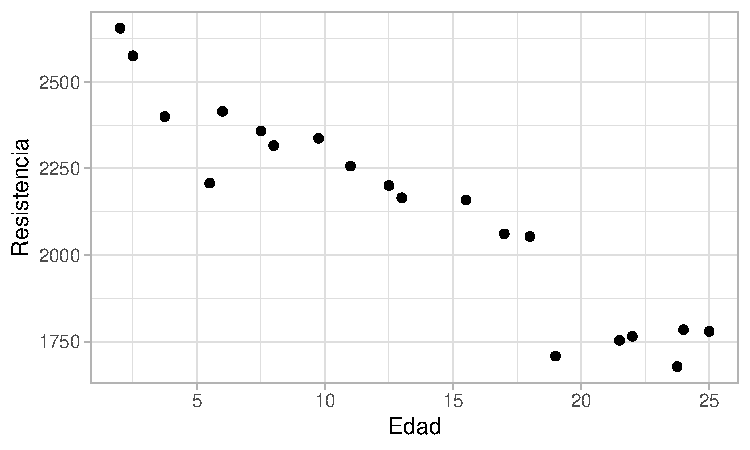
\includegraphics{libro_mod_pred_files/figure-latex/soldadura1-1} \end{center}

De la figura anterior se ve claramente que a medida que aumenta la edad de la soldadura, la resistencia que ella ofrece disminuye. Adicionalmente, se observa que la relación entre las variables es lineal con una dispersión que parece constante.

¿Quién estima mejor? ¿un modelo de regresión lineal simple o un árbol?

\begin{Shaded}
\begin{Highlighting}[]
\NormalTok{rls <-}\StringTok{ }\KeywordTok{lm}\NormalTok{(Resistencia }\OperatorTok{~}\StringTok{ }\NormalTok{Edad, }\DataTypeTok{data=}\NormalTok{datos)}
\NormalTok{arb <-}\StringTok{ }\KeywordTok{rpart}\NormalTok{(Resistencia }\OperatorTok{~}\StringTok{ }\NormalTok{Edad, }\DataTypeTok{data=}\NormalTok{datos)}
\end{Highlighting}
\end{Shaded}

\begin{Shaded}
\begin{Highlighting}[]
\NormalTok{arb <-}\StringTok{ }\KeywordTok{rpart}\NormalTok{(Resistencia }\OperatorTok{~}\StringTok{ }\NormalTok{Edad, }\DataTypeTok{data=}\NormalTok{datos, }\DataTypeTok{method=}\StringTok{"anova"}\NormalTok{)}
\end{Highlighting}
\end{Shaded}

¿Qué hay dentro de modelo de regresión lineal simple?

\begin{Shaded}
\begin{Highlighting}[]
\KeywordTok{summary}\NormalTok{(rls)}
\end{Highlighting}
\end{Shaded}

\begin{verbatim}
## 
## Call:
## lm(formula = Resistencia ~ Edad, data = datos)
## 
## Residuals:
##     Min      1Q  Median      3Q     Max 
## -215.98  -50.68   28.74   66.61  106.76 
## 
## Coefficients:
##             Estimate Std. Error t value Pr(>|t|)    
## (Intercept) 2627.822     44.184   59.48  < 2e-16 ***
## Edad         -37.154      2.889  -12.86 1.64e-10 ***
## ---
## Signif. codes:  0 '***' 0.001 '**' 0.01 '*' 0.05 '.' 0.1 ' ' 1
## 
## Residual standard error: 96.11 on 18 degrees of freedom
## Multiple R-squared:  0.9018, Adjusted R-squared:  0.8964 
## F-statistic: 165.4 on 1 and 18 DF,  p-value: 1.643e-10
\end{verbatim}

¿Qué hay dentro de modelo del arbol?

\begin{Shaded}
\begin{Highlighting}[]
\KeywordTok{summary}\NormalTok{(arb)}
\end{Highlighting}
\end{Shaded}

\begin{verbatim}
## Call:
## rpart(formula = Resistencia ~ Edad, data = datos, method = "anova")
##   n= 20 
## 
##          CP nsplit rel error   xerror      xstd
## 1 0.7480619      0 1.0000000 1.057314 0.2269184
## 2 0.0100000      1 0.2519381 1.057314 0.2269184
## 
## Variable importance
## Edad 
##  100 
## 
## Node number 1: 20 observations,    complexity param=0.7480619
##   mean=2131.358, MSE=84686.88 
##   left son=2 (8 obs) right son=3 (12 obs)
##   Primary splits:
##       Edad < 16.25 to the right, improve=0.7480619, (0 missing)
## 
## Node number 2: 8 observations
##   mean=1823.094, MSE=19439.95 
## 
## Node number 3: 12 observations
##   mean=2336.867, MSE=22599.79
\end{verbatim}

Construyamos nuevamente el árbol pero explorando todas las opciones de la función \texttt{prp}.

\begin{Shaded}
\begin{Highlighting}[]
\KeywordTok{prp}\NormalTok{(arb, }\DataTypeTok{main =} \StringTok{""}\NormalTok{,}
    \DataTypeTok{nn =} \OtherTok{TRUE}\NormalTok{,             }\CommentTok{# display the node numbers}
    \DataTypeTok{fallen.leaves =} \OtherTok{TRUE}\NormalTok{,  }\CommentTok{# put the leaves on the bottom of the page}
    \DataTypeTok{shadow.col =} \StringTok{"gray"}\NormalTok{,   }\CommentTok{# shadows under the leaves}
    \DataTypeTok{branch.lty =} \DecValTok{3}\NormalTok{,        }\CommentTok{# draw branches using dotted lines}
    \DataTypeTok{branch =} \FloatTok{.5}\NormalTok{,           }\CommentTok{# change angle of branch lines}
    \DataTypeTok{faclen =} \DecValTok{0}\NormalTok{,            }\CommentTok{# faclen = 0 to print full factor names}
    \DataTypeTok{trace =} \DecValTok{1}\NormalTok{,             }\CommentTok{# print the auto calculated cex, xlim, ylim}
    \DataTypeTok{split.cex =} \FloatTok{1.2}\NormalTok{,       }\CommentTok{# make the split text larger than the node text}
    \DataTypeTok{split.prefix =} \StringTok{"is "}\NormalTok{,  }\CommentTok{# put "is " before split text}
    \DataTypeTok{split.suffix =} \StringTok{"?"}\NormalTok{,    }\CommentTok{# put "?" after split text}
    \DataTypeTok{split.box.col =} \StringTok{"lightblue"}\NormalTok{,   }\CommentTok{# lightgray split boxes (default is white)}
    \DataTypeTok{split.border.col =} \StringTok{"darkgray"}\NormalTok{, }\CommentTok{# darkgray border on split boxes}
    \DataTypeTok{split.round =} \FloatTok{0.5}\NormalTok{)             }\CommentTok{# round the split box corners a tad}
\end{Highlighting}
\end{Shaded}

\begin{verbatim}
## cex 1   xlim c(-0.65, 1.65)   ylim c(-0.15, 1.15)
\end{verbatim}

\begin{center}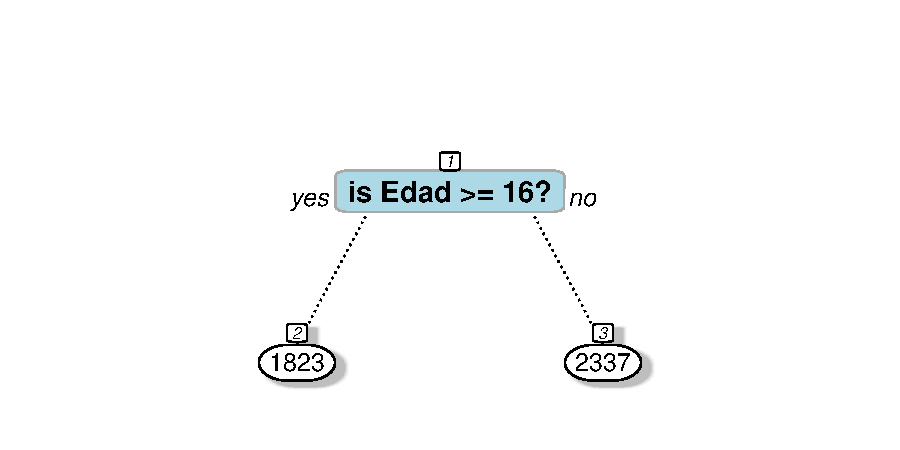
\includegraphics{libro_mod_pred_files/figure-latex/reg_arb01-1} \end{center}

A continuación las predicciones con ambos modelos.

\begin{Shaded}
\begin{Highlighting}[]
\NormalTok{pred_rls <-}\StringTok{ }\KeywordTok{predict}\NormalTok{(}\DataTypeTok{object=}\NormalTok{rls, }\DataTypeTok{newdata=}\NormalTok{datos)}
\NormalTok{pred_arb <-}\StringTok{ }\KeywordTok{predict}\NormalTok{(}\DataTypeTok{object=}\NormalTok{arb, }\DataTypeTok{newdata=}\NormalTok{datos)}
\end{Highlighting}
\end{Shaded}

Dibujemos \(y_i\) versus \(\hat{y}_i\).

\begin{Shaded}
\begin{Highlighting}[]
\KeywordTok{par}\NormalTok{(}\DataTypeTok{mfrow=}\KeywordTok{c}\NormalTok{(}\DecValTok{1}\NormalTok{, }\DecValTok{2}\NormalTok{))}
\KeywordTok{plot}\NormalTok{(}\DataTypeTok{x=}\NormalTok{pred_rls, }\DataTypeTok{y=}\NormalTok{datos}\OperatorTok{$}\NormalTok{Resistencia, }\DataTypeTok{main=}\StringTok{"RLS"}\NormalTok{)}
\KeywordTok{abline}\NormalTok{(}\DataTypeTok{a=}\DecValTok{0}\NormalTok{, }\DataTypeTok{b=}\DecValTok{1}\NormalTok{, }\DataTypeTok{lty=}\StringTok{"dashed"}\NormalTok{, }\DataTypeTok{col=}\StringTok{"blue"}\NormalTok{)}
\KeywordTok{plot}\NormalTok{(}\DataTypeTok{x=}\NormalTok{pred_arb, }\DataTypeTok{y=}\NormalTok{datos}\OperatorTok{$}\NormalTok{Resistencia, }\DataTypeTok{main=}\StringTok{"Arbol"}\NormalTok{)}
\KeywordTok{abline}\NormalTok{(}\DataTypeTok{a=}\DecValTok{0}\NormalTok{, }\DataTypeTok{b=}\DecValTok{1}\NormalTok{, }\DataTypeTok{lty=}\StringTok{"dashed"}\NormalTok{, }\DataTypeTok{col=}\StringTok{"blue"}\NormalTok{)}
\end{Highlighting}
\end{Shaded}

\begin{center}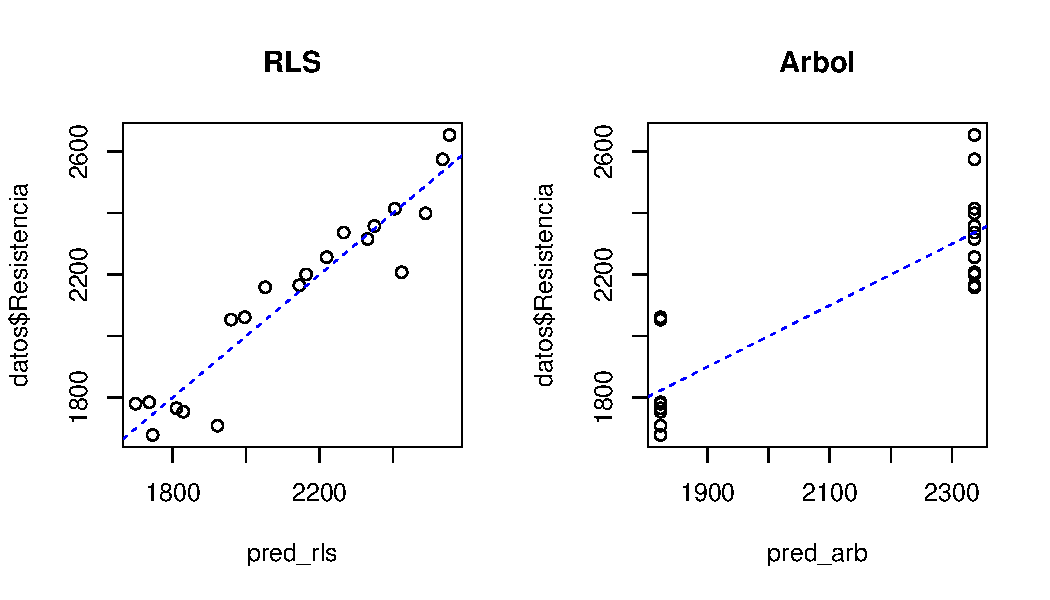
\includegraphics{libro_mod_pred_files/figure-latex/reg_arb02-1} \end{center}

Vamos a calcular \(Cor(y_i, \hat{y}_i)\).

\begin{Shaded}
\begin{Highlighting}[]
\KeywordTok{cor}\NormalTok{(datos}\OperatorTok{$}\NormalTok{Resistencia, pred_rls)}
\end{Highlighting}
\end{Shaded}

\begin{verbatim}
## [1] 0.9496533
\end{verbatim}

\begin{Shaded}
\begin{Highlighting}[]
\KeywordTok{cor}\NormalTok{(datos}\OperatorTok{$}\NormalTok{Resistencia, pred_arb)}
\end{Highlighting}
\end{Shaded}

\begin{verbatim}
## [1] 0.8649057
\end{verbatim}

Calculemos ahora el Error Cuadrático Medio \(ECM=\frac{1}{n}\sum(y_i-\hat{y}_i)^2\).

\begin{Shaded}
\begin{Highlighting}[]
\KeywordTok{mean}\NormalTok{((datos}\OperatorTok{$}\NormalTok{Resistencia }\OperatorTok{-}\StringTok{ }\NormalTok{pred_rls)}\OperatorTok{^}\DecValTok{2}\NormalTok{)}
\end{Highlighting}
\end{Shaded}

\begin{verbatim}
## [1] 8312.743
\end{verbatim}

\begin{Shaded}
\begin{Highlighting}[]
\KeywordTok{mean}\NormalTok{((datos}\OperatorTok{$}\NormalTok{Resistencia }\OperatorTok{-}\StringTok{ }\NormalTok{pred_arb)}\OperatorTok{^}\DecValTok{2}\NormalTok{)}
\end{Highlighting}
\end{Shaded}

\begin{verbatim}
## [1] 21335.85
\end{verbatim}

¿Cuál método prefiere usted?

\hypertarget{estudio-de-simulacion-para-comparar-ambos-metodos}{%
\section*{Estudio de simulación para comparar ambos métodos}\label{estudio-de-simulacion-para-comparar-ambos-metodos}}
\addcontentsline{toc}{section}{Estudio de simulación para comparar ambos métodos}

El objetivo es comparar ambos modelos repetidas veces, para esto vamos a simular conjuntos de datos que tengan un comportamiento lineal y parecido a los datos del ejemplo. El modelo que vamos a considerar es el siguiente:

\begin{align}
y_i &\sim N(\mu_i, \sigma^2), \\ 
\mu_i &= 2627 - 37 x_i, \\
\sigma &= 96, \\
x &\sim U(2, 25)
\end{align}

Vamos a crear una función generadora de datos.

\begin{Shaded}
\begin{Highlighting}[]
\NormalTok{gen_dat <-}\StringTok{ }\ControlFlowTok{function}\NormalTok{(n) \{}
\NormalTok{  x <-}\StringTok{ }\KeywordTok{runif}\NormalTok{(}\DataTypeTok{n=}\NormalTok{n, }\DataTypeTok{min=}\DecValTok{2}\NormalTok{, }\DataTypeTok{max=}\DecValTok{25}\NormalTok{)}
\NormalTok{  media <-}\StringTok{ }\DecValTok{2627} \OperatorTok{-}\StringTok{ }\DecValTok{37} \OperatorTok{*}\StringTok{ }\NormalTok{x}
\NormalTok{  y <-}\StringTok{ }\KeywordTok{rnorm}\NormalTok{(}\DataTypeTok{n=}\NormalTok{n, }\DataTypeTok{mean=}\NormalTok{media, }\DataTypeTok{sd=}\DecValTok{96}\NormalTok{)}
  \KeywordTok{data.frame}\NormalTok{(}\DataTypeTok{x=}\NormalTok{x, }\DataTypeTok{y=}\NormalTok{y)}
\NormalTok{\}}
\end{Highlighting}
\end{Shaded}

Generemos unos datos de prueba y graficamos los datos.

\begin{Shaded}
\begin{Highlighting}[]
\NormalTok{datos_train <-}\StringTok{ }\KeywordTok{gen_dat}\NormalTok{(}\DataTypeTok{n=}\DecValTok{20}\NormalTok{)}
\KeywordTok{ggplot}\NormalTok{(datos_train, }\KeywordTok{aes}\NormalTok{(}\DataTypeTok{x=}\NormalTok{x, }\DataTypeTok{y=}\NormalTok{y)) }\OperatorTok{+}\StringTok{ }
\StringTok{  }\KeywordTok{geom_point}\NormalTok{() }\OperatorTok{+}\StringTok{ }\KeywordTok{theme_light}\NormalTok{()}
\end{Highlighting}
\end{Shaded}

\begin{center}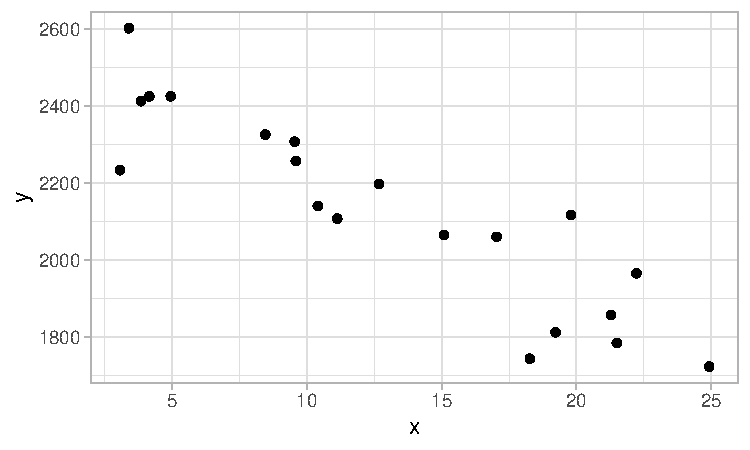
\includegraphics{libro_mod_pred_files/figure-latex/reg_arb03-1} \end{center}

Usando los datos de prueba vamos a ajustar los modelos y luego calcularemos los indicadores.

\begin{Shaded}
\begin{Highlighting}[]
\NormalTok{datos_train <-}\StringTok{ }\KeywordTok{gen_dat}\NormalTok{(}\DataTypeTok{n=}\DecValTok{20}\NormalTok{)  }\CommentTok{# Para entrenar}
\NormalTok{datos_test  <-}\StringTok{ }\KeywordTok{gen_dat}\NormalTok{(}\DataTypeTok{n=}\DecValTok{20}\NormalTok{)  }\CommentTok{# Para validar}
\NormalTok{rls <-}\StringTok{ }\KeywordTok{lm}\NormalTok{(y }\OperatorTok{~}\StringTok{ }\NormalTok{x, }\DataTypeTok{data=}\NormalTok{datos_train)}
\NormalTok{arb <-}\StringTok{ }\KeywordTok{rpart}\NormalTok{(y }\OperatorTok{~}\StringTok{ }\NormalTok{x, }\DataTypeTok{data=}\NormalTok{datos_train)}
\NormalTok{pred_rls <-}\StringTok{ }\KeywordTok{predict}\NormalTok{(}\DataTypeTok{object=}\NormalTok{rls, }\DataTypeTok{newdata=}\NormalTok{datos_test)}
\NormalTok{pred_arb <-}\StringTok{ }\KeywordTok{predict}\NormalTok{(}\DataTypeTok{object=}\NormalTok{arb, }\DataTypeTok{newdata=}\NormalTok{datos_test)}
\KeywordTok{cor}\NormalTok{(datos_test}\OperatorTok{$}\NormalTok{y, pred_rls)}
\end{Highlighting}
\end{Shaded}

\begin{verbatim}
## [1] 0.9615395
\end{verbatim}

\begin{Shaded}
\begin{Highlighting}[]
\KeywordTok{cor}\NormalTok{(datos_test}\OperatorTok{$}\NormalTok{y, pred_arb)}
\end{Highlighting}
\end{Shaded}

\begin{verbatim}
## [1] 0.8500365
\end{verbatim}

\begin{Shaded}
\begin{Highlighting}[]
\KeywordTok{mean}\NormalTok{((datos_test}\OperatorTok{$}\NormalTok{y }\OperatorTok{-}\StringTok{ }\NormalTok{pred_rls)}\OperatorTok{^}\DecValTok{2}\NormalTok{)}
\end{Highlighting}
\end{Shaded}

\begin{verbatim}
## [1] 8010.614
\end{verbatim}

\begin{Shaded}
\begin{Highlighting}[]
\KeywordTok{mean}\NormalTok{((datos_test}\OperatorTok{$}\NormalTok{y }\OperatorTok{-}\StringTok{ }\NormalTok{pred_arb)}\OperatorTok{^}\DecValTok{2}\NormalTok{)}
\end{Highlighting}
\end{Shaded}

\begin{verbatim}
## [1] 23925.86
\end{verbatim}

\BeginKnitrBlock{rmdwarning}
Al observar los resultados anteriores vemos que el modelo de regresión lineal se comporta mejor que el árbol de regresión, esto se debe a que los datos están siendo generados con un modelo de regresión lineal.
\EndKnitrBlock{rmdwarning}

Ahora vamos a realizar el estudio de simulación para explorar el efecto de \(n = 10, 20, 40\) sobre el \(ECM\) usando 5 réplicas para cada \(n\), este es un estudio de simulación ``naive'' pero ilustrativo.

\begin{Shaded}
\begin{Highlighting}[]
\NormalTok{n <-}\StringTok{ }\KeywordTok{c}\NormalTok{(}\DecValTok{10}\NormalTok{, }\DecValTok{20}\NormalTok{, }\DecValTok{40}\NormalTok{)}
\NormalTok{nrep <-}\StringTok{ }\DecValTok{5}
\NormalTok{result <-}\StringTok{ }\KeywordTok{numeric}\NormalTok{()}
\ControlFlowTok{for}\NormalTok{ (i }\ControlFlowTok{in}\NormalTok{ n) \{}
  \ControlFlowTok{for}\NormalTok{(k }\ControlFlowTok{in} \DecValTok{1}\OperatorTok{:}\NormalTok{nrep) \{}
\NormalTok{    datos_train <-}\StringTok{ }\KeywordTok{gen_dat}\NormalTok{(}\DataTypeTok{n=}\NormalTok{i)  }\CommentTok{# Para entrenar}
\NormalTok{    datos_test  <-}\StringTok{ }\KeywordTok{gen_dat}\NormalTok{(}\DataTypeTok{n=}\NormalTok{i)  }\CommentTok{# Para validar}
\NormalTok{    rls <-}\StringTok{ }\KeywordTok{lm}\NormalTok{(y }\OperatorTok{~}\StringTok{ }\NormalTok{x, }\DataTypeTok{data=}\NormalTok{datos_train)}
\NormalTok{    arb <-}\StringTok{ }\KeywordTok{rpart}\NormalTok{(y }\OperatorTok{~}\StringTok{ }\NormalTok{x, }\DataTypeTok{data=}\NormalTok{datos_train)}
\NormalTok{    pred_rls <-}\StringTok{ }\KeywordTok{predict}\NormalTok{(}\DataTypeTok{object=}\NormalTok{rls, }\DataTypeTok{newdata=}\NormalTok{datos_test)}
\NormalTok{    pred_arb <-}\StringTok{ }\KeywordTok{predict}\NormalTok{(}\DataTypeTok{object=}\NormalTok{arb, }\DataTypeTok{newdata=}\NormalTok{datos_test)}
\NormalTok{    ecm1 <-}\StringTok{ }\KeywordTok{mean}\NormalTok{((datos_test}\OperatorTok{$}\NormalTok{y }\OperatorTok{-}\StringTok{ }\NormalTok{pred_rls)}\OperatorTok{^}\DecValTok{2}\NormalTok{)}
\NormalTok{    ecm2 <-}\StringTok{ }\KeywordTok{mean}\NormalTok{((datos_test}\OperatorTok{$}\NormalTok{y }\OperatorTok{-}\StringTok{ }\NormalTok{pred_arb)}\OperatorTok{^}\DecValTok{2}\NormalTok{)}
\NormalTok{    result <-}\StringTok{ }\KeywordTok{rbind}\NormalTok{(result, }\KeywordTok{c}\NormalTok{(i, ecm1, ecm2)) }\CommentTok{# No eficiente pero sirve}
\NormalTok{  \}}
\NormalTok{\}}
\KeywordTok{colnames}\NormalTok{(result) <-}\StringTok{ }\KeywordTok{c}\NormalTok{(}\StringTok{"n"}\NormalTok{, }\StringTok{"ecm_lrs"}\NormalTok{, }\StringTok{"ecm_arb"}\NormalTok{)}
\NormalTok{result <-}\StringTok{ }\KeywordTok{as.data.frame}\NormalTok{(result)}
\NormalTok{result}
\end{Highlighting}
\end{Shaded}

\begin{verbatim}
##     n   ecm_lrs   ecm_arb
## 1  10 22342.892  67143.51
## 2  10 28186.080 109455.80
## 3  10 18074.550  72013.92
## 4  10  5747.585  79585.71
## 5  10 12592.402  60357.27
## 6  20  7624.788  27244.90
## 7  20  7825.550  29318.18
## 8  20  5721.970  20488.30
## 9  20  9683.974  32764.16
## 10 20 13750.203  21107.22
## 11 40  8436.121  27969.58
## 12 40 12162.325  20550.88
## 13 40 14748.927  14208.98
## 14 40  9615.399  22187.77
## 15 40 11055.010  14160.77
\end{verbatim}

El objeto \texttt{result} tiene los resultados de la simulación, vamos a calcular el \(ECM\) promedio para rls y árboles diferenciando por \(n\).

\begin{Shaded}
\begin{Highlighting}[]
\KeywordTok{library}\NormalTok{(dplyr)}
\NormalTok{result }\OperatorTok\StringTok{ }\KeywordTok{group_by}\NormalTok{(n) }\OperatorTok\StringTok{ }\KeywordTok{summarise}\NormalTok{(}\DataTypeTok{ecm_medio_lrs=}\KeywordTok{mean}\NormalTok{(ecm_lrs),}
                                     \DataTypeTok{ecm_medio_arb=}\KeywordTok{mean}\NormalTok{(ecm_arb))}
\end{Highlighting}
\end{Shaded}

\begin{verbatim}
## # A tibble: 3 x 3
##       n ecm_medio_lrs ecm_medio_arb
##   <dbl>         <dbl>         <dbl>
## 1    10        17389.        77711.
## 2    20         8921.        26185.
## 3    40        11204.        19816.
\end{verbatim}

\hypertarget{retos}{%
\section*{Retos}\label{retos}}
\addcontentsline{toc}{section}{Retos}

A continuación los retos que usted debe aceptar.

\begin{enumerate}
\def\labelenumi{\arabic{enumi}.}
\tightlist
\item
  Extienda el estudio de simulación para otros valores de \(n\) y aumentando el número de repeticiones \texttt{nrep}, decida usted los valores.
\item
  Con los resultados anteriores haga un gráfico de \(ECM\) promedio versus \(n\) para rls y árboles en la misma figura.
\item
  ¿Se iguala \(ECM\) promedio del árbol con el de regresión para algún valor de \(n\)?
\item
  ¿Cuál técnica presenta el \(ECM\) menor?
\item
  ¿Es posible encontrar un \(ECM=0\) para algún valor de \(n\)?
\item
  ¿Para qué sirve el paquete \texttt{dplyr}?
\item
  ¿Qué es un \texttt{tibble}?
\end{enumerate}

\bibliography{book.bib,packages.bib}

\backmatter
\printindex


\end{document}
